% CVPR 2027 review manuscript. Official cvpr.sty is kept unchanged.
\documentclass[10pt,twocolumn,letterpaper]{article}
\usepackage[T1]{fontenc}
\usepackage[review]{cvpr}
\usepackage{amsmath,amssymb,amsthm}
\usepackage{booktabs,multirow,graphicx}
\usepackage{tikz}
\usetikzlibrary{arrows.meta,positioning,calc}
\definecolor{cvprblue}{rgb}{0.21,0.49,0.74}
\usepackage[pagebackref,breaklinks,colorlinks,allcolors=cvprblue]{hyperref}
\def\confName{CVPR}
\def\confYear{2027}
\newcommand{\method}{NBP}
\newcommand{\R}{\mathbb{R}}
\newtheorem{proposition}{Proposition}
\title{Nullspace Bias Perturbation for Post-hoc Model Merge Protection}
\author{Anonymous authors}
\begin{document}
\maketitle
\begin{abstract}
Open-weight experts can be reused through parameter merging without the provider's permission. A useful release-time protection should preserve the expert's standalone function while disrupting its contribution after merging. We study a simple construction for CLIP vision encoders. Nullspace Bias Perturbation (\method) changes only the bias of the final LayerNorm. The added vector lies in the left nullspace of the expert's visual projection, so its contribution vanishes in the original encoder. Parameter merging changes this projection and can expose the perturbation. We choose the direction and magnitude from frozen weights and a fixed classifier, without images or optimization. A LayerNorm norm bound gives a sufficient condition for a constant prediction in a public-base interpolation model. Across 42 directed pairs of seven classification tasks, NBP changes standalone accuracy by less than 0.03 percentage points and reduces mean target accuracy after AGA and merging from 84.81\% to 3.30\%. Tests also cover eight-expert merging, two additional fusion rules, and a second vision backbone. Public final-MLP replacement and fixed block-wise coefficient fitting leave the effect intact on three tested tasks. A projection of the final bias removes it, which limits the protection to procedures that retain that readout.
\end{abstract}

\section{Introduction}
Model merging combines independently fine-tuned experts without joint training. Task Arithmetic adds their updates relative to a shared pretrained checkpoint~\cite{ilharco2023task}; other methods prune or resolve conflicting updates before combination~\cite{yadav2023ties,yu2024dare}. This makes released weights useful beyond their original deployment. It also allows a downstream user to combine an expert's capabilities into another model without authorization.

Release-time merge protection aims to preserve normal use of an expert while reducing its usefulness in such combinations. PaRaMS transforms MLP and attention parameters without changing their functions~\cite{wei2025params}. Later defenses use structural changes, additional training, or weight perturbations~\cite{li2025mergebarrier,chen2026mergeguard,jang2026trap2}. These approaches illustrate the difference between functional and parameter equivalence. Two parameterizations can implement the same expert yet behave differently when their parameters are averaged.

The recovery procedure is equally important. AGA aligns protected weights to a public checkpoint and can reverse transformations that affect selected MLP and attention modules~\cite{guo2026aga}. A large parameter displacement alone therefore does not establish protection. Evaluation must state which parameters the recovery procedure modifies and measure the resulting merged model on complete test sets.

We consider one location where standalone and merged behavior can be separated algebraically. A CLIP vision encoder ends with a LayerNorm and a rectangular visual projection~\cite{radford2021clip}. A bias vector in the left nullspace of this projection has zero effect on the encoder's output. When the projection itself is merged with another model, the same vector need not remain in its nullspace. We use this change to construct Nullspace Bias Perturbation (\method).

The construction changes one bias vector. Its direction is computed inside the exact projection nullspace, and its magnitude is obtained from a bound on normalized LayerNorm features. Both depend only on frozen model weights and the classifier. There is no construction dataset, optimizer, or update to the original expert. The preservation identity holds in exact arithmetic for every input; finite-precision changes are measured separately.

We make three contributions. First, we give an image-free construction that changes a single bias while preserving the complete standalone embedding in exact arithmetic. Second, we derive how task arithmetic exposes this update and a sufficient condition for constant predictions from the final readout alone. Third, we evaluate standalone utility, merging and recovery using matched controls on seven tasks, and test a second vision backbone. A public projection of the final bias removes the added component, establishing an explicit boundary of this construction.

\begin{table*}[!t]
\centering
\small
\setlength{\tabcolsep}{4pt}
\caption{Standalone and protected-task accuracy (\%) with matched checkpoints and processing. Bold scores mark the lowest merged accuracy per setting. TA coefficients are 0.5 for two experts and 0.2 for eight experts. Avg. is the unweighted mean of the seven displayed task scores. Companions are SVHN for MNIST and MNIST otherwise. EuroSAT participates in eight-expert merging.}
\label{tab:main}
\begin{tabular}{llrrrrrrrr}
\toprule
Setting & Defense & SUN397 & Cars & RESISC45 & SVHN & GTSRB & MNIST & DTD & Avg. \\
\midrule
\multirow{3}{*}{Standalone} & None & 75.28 & 77.66 & 96.11 & 97.46 & 98.73 & 99.69 & 79.41 & 89.19 \\
 & PaRaMS & 75.28 & 77.66 & 96.11 & 97.46 & 98.73 & 99.69 & 79.41 & 89.19 \\
 & \textbf{NBP} & 75.27 & 77.64 & 96.11 & 97.46 & 98.73 & 99.69 & 79.41 & 89.19 \\
\midrule
\multirow{3}{*}{2-expert TA} & None & 71.92 & 73.17 & 91.08 & 92.50 & 93.25 & 99.37 & 69.31 & 84.37 \\
 & PaRaMS & 0.30 & 0.72 & 2.57 & 9.09 & 2.79 & \textbf{8.92} & \textbf{2.07} & 3.78 \\
 & \textbf{NBP} & \textbf{0.25} & \textbf{0.55} & \textbf{2.44} & \textbf{6.70} & \textbf{1.19} & 9.80 & 2.13 & \textbf{3.29} \\
\midrule
\multirow{3}{*}{2-expert AGA + TA} & None & 71.58 & 72.53 & 90.38 & 91.56 & 92.22 & 99.30 & 68.40 & 83.71 \\
 & PaRaMS & 71.58 & 72.53 & 90.37 & 91.56 & 92.22 & 99.30 & 68.35 & 83.70 \\
 & \textbf{NBP} & \textbf{0.25} & \textbf{0.55} & \textbf{2.44} & \textbf{6.70} & \textbf{1.19} & \textbf{9.80} & \textbf{2.13} & \textbf{3.29} \\
\midrule
\multirow{3}{*}{8-expert TA} & None & 63.76 & 62.06 & 72.00 & 74.42 & 65.08 & 94.00 & 52.18 & 69.07 \\
 & PaRaMS & 0.28 & \textbf{0.55} & 2.70 & 9.71 & 1.77 & 9.82 & \textbf{2.13} & 3.85 \\
 & \textbf{NBP} & \textbf{0.25} & \textbf{0.55} & \textbf{2.44} & \textbf{6.70} & \textbf{1.19} & \textbf{9.80} & \textbf{2.13} & \textbf{3.29} \\
\midrule
\multirow{3}{*}{8-expert AGA + TA} & None & 63.56 & 61.61 & 71.46 & 72.53 & 63.29 & 93.23 & 51.38 & 68.15 \\
 & PaRaMS & 63.56 & 61.61 & 71.46 & 72.53 & 63.29 & 93.23 & 51.38 & 68.15 \\
 & \textbf{NBP} & \textbf{0.25} & \textbf{0.55} & \textbf{2.44} & \textbf{6.70} & \textbf{1.19} & \textbf{9.80} & \textbf{2.13} & \textbf{3.29} \\
\bottomrule
\end{tabular}
\end{table*}

\section{Related Work}
\paragraph{Model merging.}
Task Arithmetic combines task vectors relative to a shared initialization~\cite{ilharco2023task}. TIES removes small updates and resolves sign conflicts~\cite{yadav2023ties}, while DARE applies randomized dropping and rescaling~\cite{yu2024dare}. ProDistill progressively fits element-wise merging coefficients using layer outputs~\cite{xu2025prodistill}. We distinguish these fusion rules from recovery operations applied before or after merging.

\paragraph{Protection against merging.}
PaRaMS uses MLP permutation and attention scaling~\cite{wei2025params}. MergeBarrier changes FFN computation and transforms attention parameters~\cite{li2025mergebarrier}. MergeGuard combines regularized training with task-vector perturbation~\cite{chen2026mergeguard}. Trap$^2$ trains updates to be accurate at their nominal scale and inaccurate at other scales~\cite{jang2026trap2}. Our construction instead changes a final normalization bias in the kernel of the expert's output projection. Its preservation argument does not require training or representative inputs.

\paragraph{Alignment and recovery.}
AGA estimates alignment to a public pretrained reference~\cite{guo2026aga}. Recovery need not reconstruct the original weights if it can recover the desired function. Public-module substitution and distillation therefore address different conditions from alignment alone. We identify the modified modules, data access, and optimization variables for each reported procedure. ProDistill remains a model-merging algorithm in this comparison; its fixed layer-wise fitting procedure is used as a recovery check.

\paragraph{Nullspace invariance.}
Adding a vector in a linear map's kernel leaves its output unchanged. This is a standard linear-algebra identity. Nullspaces have also been used for model watermark verification, including output-space invariants in NSmark~\cite{zhao2024nsmark}. Such a shared mathematical tool does not by itself establish a new protection mechanism. The distinction studied here is a frozen-parameter bias update that is invisible under the expert's own projection and becomes visible when that projection is merged. We make no claim to have introduced nullspace projection itself.

\section{Nullspace Bias Perturbation}
\label{sec:method}
\subsection{Setting and notation}
Let $\theta_0$ be a public pretrained checkpoint and $\theta_e$ a fine-tuned expert. The defender publishes a modified checkpoint $\theta_e'$ and seeks to retain standalone utility while reducing protected-task utility after parameter merging. Construction uses only $\theta_0$, $\theta_e$, and a fixed task classifier. The defender does not inspect a partner checkpoint or task images.

The downstream user has the released checkpoint and the public base. We test direct merging and published recovery procedures, and separately examine a method-specific readout cleanup. Our objective is to disrupt unauthorized merging; it does not require preserving companion-task accuracy in the merged model. The released expert must retain its standalone function.

Write the final visual embedding of the expert as
\begin{equation}
 t_e(x)=[z_e(x)\operatorname{diag}(\gamma_e)+b_e^{\mathsf T}]P_e,
 \label{eq:embedding}
\end{equation}
Here $P_e\in\R^{d\times p}$ is the visual projection. Hidden features $z_e\in\R^{1\times d}$ and embeddings $t_e\in\R^{1\times p}$ are row vectors; $b_e,\gamma_e\in\R^d$ are column vectors. The features $z_e$ are centered and variance-normalized before the learned LayerNorm affine transformation. For the evaluated ViT-B/32 and ViT-B/16 encoders, $d=768$, $p=512$, and $P_e$ has full column rank. With the usual positive LayerNorm epsilon,
\begin{equation}
 z_e\mathbf{1}_d=0,\qquad \|z_e\|_2\leq\sqrt d.
 \label{eq:lnbound}
\end{equation}
The classifier uses fixed class vectors $w_j\in\R^p$, zero class biases and a shared positive scale $\eta$:
\begin{equation}
 s_j(x)=\eta\,\frac{t_e(x)w_j}{\|t_e(x)\|_2}.
 \label{eq:cosine}
\end{equation}
For nonzero embeddings, class comparisons therefore depend only on the signs of $t_e(x)(w_k-w_j)$.

\begin{figure}[!t]
\centering
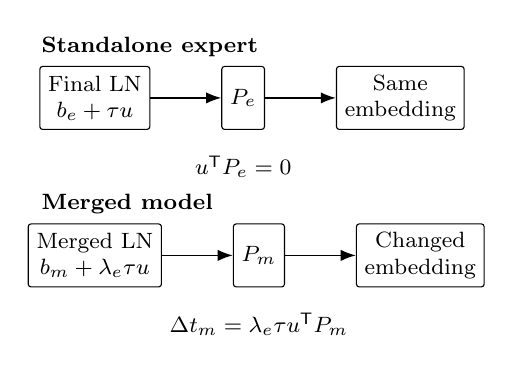
\begin{tikzpicture}[font=\footnotesize,>=Latex,
 node distance=5mm,
 box/.style={draw,rounded corners=1pt,align=center,minimum height=8mm,inner sep=3pt},
 arr/.style={->,line width=.55pt}]
\node[anchor=west] at (-.15,2.8) {\textbf{Standalone expert}};
\node[box] (ln) at (.65,2.15) {Final LN\\$b_e+\tau u$};
\node[box,right=9mm of ln] (proj) {$P_e$};
\node[box,right=9mm of proj] (out) {Same\\embedding};
\draw[arr] (ln)--(proj);
\draw[arr] (proj)--(out);
\node[below=2mm of proj,align=center] {$u^{\mathsf T}P_e=0$};
\node[anchor=west] at (-.15,.8) {\textbf{Merged model}};
\node[box] (mln) at (.65,.15) {Merged LN\\$b_m+\lambda_e\tau u$};
\node[box,right=9mm of mln] (mproj) {$P_m$};
\node[box,right=9mm of mproj] (mout) {Changed\\embedding};
\draw[arr] (mln)--(mproj);
\draw[arr] (mproj)--(mout);
\node[below=2mm of mproj,align=center] {$\Delta t_m=\lambda_e\tau u^{\mathsf T}P_m$};
\end{tikzpicture}
\caption{The bias perturbation vanishes under the expert's own projection. Merging changes the projection and can expose a constant feature offset. The actual classification effect is measured for each fusion rule and partner. This is a structural illustration.}
\label{fig:mechanism}
\end{figure}

\subsection{Preserving the standalone encoder}
Let $N_e\in\R^{d\times(d-p)}$ be an orthonormal basis of $\ker(P_e^{\mathsf T})$. As shown in \cref{fig:mechanism}, choose $u=N_ea$ and publish
\begin{equation}
 b_e'=b_e+\tau u,\qquad \tau>0,
 \label{eq:bias}
\end{equation}
leaving all other parameters unchanged.

\begin{proposition}[Standalone preservation]
If $P_e^{\mathsf T}u=0$, then the modification in \cref{eq:bias} preserves the visual embedding in exact arithmetic for every input.
\end{proposition}
\begin{proof}
The LayerNorm input, mean, variance, gain, and visual projection are unchanged. Hence the embedding difference is $\tau u^{\mathsf T}P_e=0$.
\end{proof}

The identity applies to every input and any fixed head on the visual embedding. A nonzero construction requires a nontrivial left nullspace; a full-row-rank projection with $d\le p$ does not provide one. We use an SVD to compute the basis and store the released bias in FP32. This leaves the architecture and inference cost unchanged. Large bias values can increase cancellation error in floating point, which we assess on the full standalone test sets.

\subsection{Why merging can expose the perturbation}
For Task Arithmetic with coefficients $\lambda_i$, the merged checkpoint is
\begin{equation}
 \theta_m=\theta_0+\sum_i\lambda_i(\theta_i-\theta_0).
 \label{eq:ta}
\end{equation}
If expert $e$ is protected, its bias perturbation enters with coefficient $\lambda_e$. Denote the merged visual projection by $P_m$. Relative to the same merged model without this bias update, the embedding difference is exactly
\begin{equation}
 \Delta t_m(x)=\lambda_e\tau u^{\mathsf T}P_m.
 \label{eq:exposure}
\end{equation}
The offset is constant across inputs because it is added after hidden-feature normalization. To separate the available public information from the unknown partners, write $\Delta P_i=P_i-P_0$. Using $u^{\mathsf T}P_e=0$ gives
\begin{equation}
\begin{aligned}
 u^{\mathsf T}P_m
 &=u^{\mathsf T}\widetilde P(\lambda_e)+u^{\mathsf T}E,\\
 \widetilde P(\lambda_e)&=(1-\lambda_e)P_0+\lambda_eP_e,\\
 E&=\sum_{i\ne e}\lambda_i\Delta P_i.
\end{aligned}
\label{eq:partners}
\end{equation}
The first term is available before release. The second describes the contribution of the partners' task updates. This exact decomposition motivates using the public-base interpolation to choose the perturbation. It does not assume that $E$ is small. For a class contrast $v=w_k-w_j$, the discrepancy satisfies
\begin{equation}
 |u^{\mathsf T}(P_m-\widetilde P)v|
 \leq \|u\|_2\|Ev\|_2.
 \label{eq:partnererror}
\end{equation}
Thus a positive proxy offset remains positive whenever its gap exceeds this error, although a constant prediction also requires the full feature bound below. For two experts at coefficient $0.5$, the offset reduces to $\tau u^{\mathsf T}P_{\mathrm{partner}}/4$. A partner with the same left nullspace exposes no perturbation. We evaluate partner models rather than assuming a universal transfer guarantee.

\subsection{Choosing a direction without images}
We use a public-base interpolation with fixed coefficient $\lambda=0.5$ to select a direction. This interpolation uses the protected expert and the public base, without a partner expert. Denote its final parameters by $\widetilde P,\widetilde\gamma,\widetilde b$. Let $W$ contain the fixed class vectors as rows and define the centered classifier $W_c=(I_C-\mathbf{1}_C\mathbf{1}_C^{\mathsf T}/C)W$.

Compute the thin SVD
\begin{equation}
 H=N_e^{\mathsf T}\widetilde P W_c^{\mathsf T}=U\Sigma V^{\mathsf T}.
\end{equation}
A fixed seed selects a class index before evaluation. Its centered one-hot vector is $g$. Using all numerically nonzero singular directions, set
\begin{equation}
 a=U\Sigma^{\dagger}V^{\mathsf T}g,\qquad u=N_ea.
 \label{eq:direction}
\end{equation}
This is the minimum-norm least-squares solution $a=(H^{\mathsf T})^\dagger g$; $u$ is not separately normalized. It fits class offsets using weights alone. We determine the largest resulting class offset, with index $k$, and require positive gaps
\begin{equation}
 \delta_{kj}=u^{\mathsf T}\widetilde P(w_k-w_j)>0
 \quad\text{for all }j\neq k.
\end{equation}
The construction is defined for directions satisfying this condition. All seven B/32 releases satisfy it at the fixed class draw; the condition is not automatic for an arbitrary classifier.

\subsection{Choosing a magnitude from a feature bound}
For each competitor $j$, define
\begin{equation}
 q_{kj}=\widetilde P(w_k-w_j),\quad
 C_d=I_d-\mathbf{1}_d\mathbf{1}_d^{\mathsf T}/d.
\end{equation}
The class-$k$ margin numerator of the protected public-base interpolation is
\begin{equation}
 z\operatorname{diag}(\widetilde\gamma)q_{kj}
 +\widetilde b^{\mathsf T}q_{kj}
 +\lambda\tau\delta_{kj}.
 \label{eq:margin}
\end{equation}
Because $z$ is centered, \cref{eq:lnbound} bounds its first term below by $-\sqrt d\|C_d\operatorname{diag}(\widetilde\gamma)q_{kj}\|_2$.

\begin{proposition}[Sufficient proxy condition]
Suppose all $\delta_{kj}$ are positive. If
\begin{equation}
\tau > \max_{j\neq k}
\frac{[\sqrt d\|C_d\operatorname{diag}(\widetilde\gamma)q_{kj}\|_2
-\widetilde b^{\mathsf T}q_{kj}]_+}{\lambda\delta_{kj}},
\label{eq:magnitude}
\end{equation}
then class $k$ has a strictly positive margin over every competitor for every normalized hidden state in the public-base interpolation model.
\end{proposition}
\begin{proof}
Substitution of the lower bound into \cref{eq:margin} makes each pairwise margin positive. The common feature normalization does not alter their signs.
\end{proof}

We set the magnitude to twice the bound and check the positive margins after FP32 materialization. This uses the same rule for every task, with no image-based fitting. The interpolation coefficient is fixed at $0.5$ for construction, including releases later evaluated in eight-expert merging.

\subsection{Analyzing a fixed merged model}
The same feature bound can be applied to the actual merged parameters after publication. For a candidate class $k$, let $q_{kj}=P_m(w_k-w_j)$ and compute
\begin{equation}
 L_{kj}=b_m^{\mathsf T}q_{kj}
 -\sqrt d\|C_d\operatorname{diag}(\gamma_m)q_{kj}\|_2.
 \label{eq:actualbound}
\end{equation}
If $\min_{j\neq k}L_{kj}>0$, the model predicts class $k$ for every normalized hidden state in exact arithmetic. The proof follows the same centered-feature bound as \cref{eq:margin}. This conclusion holds after arbitrary changes to preceding blocks, provided the final gain, bias, projection, and classifier stay fixed. It does not cover recovery that changes those final parameters. A negative lower bound is inconclusive.

We apply this test to the stored merged readouts after release. Partner weights enter this analysis, but not the construction. The bound concerns real-arithmetic evaluation of those stored tensors.

\section{Experiments}
\label{sec:experiments}
\subsection{Setup}
We evaluate frozen CLIP ViT-B/32 experts~\cite{radford2021clip} on MNIST, SVHN, DTD, RESISC45, Cars, GTSRB, and SUN397. Complete test sets contain 10,000, 26,032, 1,880, 6,300, 8,041, 12,630, and 19,850 images, respectively. DTD uses the official test1 split. The eight-expert pool additionally contains EuroSAT; all reported task averages use the seven listed test sets.

Each two-expert experiment protects one expert and uses a fixed companion expert. MNIST uses SVHN as its companion; the other six use MNIST. Task Arithmetic uses coefficient 0.5 for each update. We compare unprotected experts, the official PaRaMS implementation with its fixed defaults, and \method. For AGA, the same author implementation processes the protected expert and the matching unprotected control before merging. It does not update the original expert through training.

Construction uses FP64 SVD with relative singular-value tolerance $10^{-10}$, a fixed random seed and the magnitude multiplier 2. Released parameters and inference use FP32. Every method uses the same checkpoints, classification heads and preprocessing. We report complete-test accuracy in percent, including companion-task accuracy. Among the procedures in \cref{tab:recovery}, only ProDistill uses training images. NBP construction uses none.

\subsection{Standalone utility and two-expert merging}
\Cref{tab:main} reports the seven protected tasks. After AGA and two-expert TA, mean target accuracy falls from 83.71\% to 3.29\% with \method{}. Five tasks retain every evaluated prediction. Cars has eight changed predictions and two net losses among 8,041 examples. SUN397 has four changed predictions and two net losses among 19,850 examples. The maximum standalone decrease is 0.025 percentage points.

Direct merging with PaRaMS or \method{} gives low target accuracy. AGA restores PaRaMS close to the unprotected control, while \method{} remains between 0.25\% and 9.80\%. AGA aligns attention and MLP parameters and leaves the final normalization bias fixed.

The loss of accuracy can be traced to a change in the prediction distribution. On MNIST, the protected AGA merge predicts digit 0 for all 10,000 examples (\cref{fig:predictions}), so its accuracy equals the test frequency of that digit, 9.80\%. The effect extends to the companion task: its mean accuracy across the seven pairs falls from 98.44\% to 15.72\% after AGA and TA (\cref{tab:partners}).

\begin{table}[!t]
\centering
\small
\setlength{\tabcolsep}{4pt}
\caption{Accuracy after AGA and TA across all 42 directed pairs (\%). Each row averages the six other validated tasks as companions. Subscripts t and c denote the protected target and companion; U is the unprotected control. The same seven NBP releases are used throughout.}
\label{tab:partners}
\begin{tabular}{lrrrr}
\toprule
Task & U$_t$ & NBP$_t$ & U$_c$ & NBP$_c$ \\
\midrule
SUN397 & 71.94 & 0.34 & 88.38 & 4.28 \\
Cars & 72.58 & 0.51 & 88.34 & 4.27 \\
RESISC45 & 91.19 & 2.44 & 84.26 & 8.17 \\
SVHN & 93.65 & 6.70 & 83.50 & 5.31 \\
GTSRB & 94.95 & 1.19 & 83.70 & 9.37 \\
MNIST & 99.30 & 9.80 & 82.12 & 2.80 \\
DTD & 70.07 & 2.13 & 88.52 & 5.86 \\
\bottomrule
\end{tabular}
\end{table}

\begin{figure}[!t]
\centering
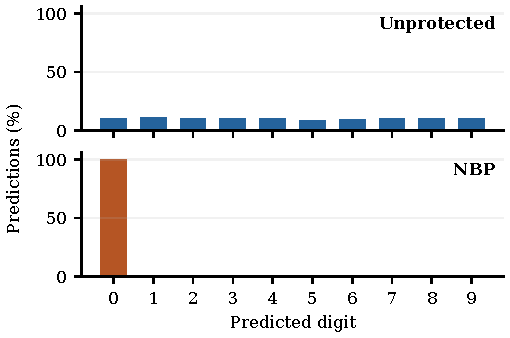
\includegraphics[width=\linewidth]{fig/predictions.pdf}
\caption{MNIST prediction frequencies after AGA and TA with the SVHN expert. The unprotected merge predicts all ten classes. With NBP, every example is assigned to digit 0.}
\label{fig:predictions}
\end{figure}

\subsection{Specified recovery procedures}
\begin{table}[!t]
\centering
\small
\setlength{\tabcolsep}{4pt}
\caption{Protected-task accuracy after the specified recovery procedures (\%). B reset replaces the final MLP output weight and bias after AGA, then applies TA. ProDistill uses its fixed layer-wise fitting protocol; final LayerNorm and projection are not optimized. The control receives the same processing.}
\label{tab:recovery}
\begin{tabular}{llrrr}
\toprule
Procedure & Defense & MNIST & SVHN & DTD \\
\midrule
\multirow{2}{*}{B reset} & None & 99.29 & 91.47 & 67.18 \\
 & \textbf{NBP} & 9.80 & 6.70 & 2.13 \\
\midrule
\multirow{3}{*}{ProDistill} & None & 99.45 & 96.73 & 73.14 \\
 & PaRaMS & 89.27 & 66.22 & 7.29 \\
 & \textbf{NBP} & 9.80 & 6.70 & 2.13 \\
\bottomrule
\end{tabular}
\end{table}

\paragraph{Public MLP replacement.}
Following the public-parameter replacement setting discussed in MergeBarrier~\cite{li2025mergebarrier}, our fixed check replaces the final MLP output matrix and its bias with the public base values. Replacement occurs after AGA and before TA. The operation is applied to both the protected model and the unprotected control. This is a native adaptation to the evaluated CLIP model, not a reproduction of the LLM experiment. Because it leaves the final LayerNorm bias unchanged, \method{} remains at 9.80\%, 6.70\%, and 2.13\% on MNIST, SVHN, and DTD.

\paragraph{Layer-wise coefficient fitting.}
We use the fixed author ProDistill kernel~\cite{xu2025prodistill}. The attacker has 64 unlabeled training images per task, task identity, and 100 coefficient-optimization steps per block, with initial coefficients 0.3. The two-expert adaptation updates element-wise block coefficients. The final LayerNorm and visual projection remain fixed throughout this procedure. The expert weights themselves are frozen. The unprotected and PaRaMS controls use the same data and fitting budget. The fits reduce PaRaMS accuracy on DTD as well as NBP accuracy, despite retaining 73.14\% in the unprotected control.

\subsection{Other fusion rules}
\begin{table}[!t]
\centering
\small
\setlength{\tabcolsep}{4pt}
\caption{Additional fusion rules on the fixed SUN397/MNIST pair (\%). TIES retains 20\% of entries with scale 1. DARE+TA uses drop rate 0.2, seed 42, and TA coefficient 0.5. AGA processes the protected expert. Both complete test sets and matching controls are reported.}
\label{tab:fusion}
\begin{tabular}{llrr}
\toprule
Fusion / recovery & Defense & SUN397 & MNIST \\
\midrule
\multirow{3}{*}{TIES} & None & 74.27 & 99.60 \\
 & PaRaMS & 0.29 & 8.92 \\
 & NBP & 0.25 & 10.28 \\
\midrule
\multirow{3}{*}{TIES + AGA} & None & 74.03 & 99.60 \\
 & PaRaMS & 74.03 & 99.60 \\
 & NBP & 0.25 & 10.28 \\
\midrule
\multirow{3}{*}{DARE+TA} & None & 71.87 & 99.45 \\
 & PaRaMS & 0.25 & 9.57 \\
 & NBP & 0.25 & 10.28 \\
\midrule
\multirow{3}{*}{DARE+TA + AGA} & None & 71.53 & 99.45 \\
 & PaRaMS & 71.53 & 99.45 \\
 & NBP & 0.25 & 10.28 \\
\bottomrule
\end{tabular}
\end{table}

\Cref{tab:fusion} evaluates the same frozen SUN397 releases with TIES and DARE+TA. TIES uses global top-20\% trimming and scale 1; DARE drops 20\% of task-update entries with fixed seed 42 before TA at 0.5. We use unchanged author kernels through the existing CLIP adapter. The settings are shared by all three defenses and are not selected from their test scores. With or without AGA, \method{} yields 50 correct SUN397 predictions out of 19,850, or 0.25\%. Companion MNIST accuracy is 10.28\%.

\subsection{Direction and magnitude}
\begin{table}[!t]
\centering
\small
\setlength{\tabcolsep}{4pt}
\caption{Direction controls on MNIST (\%). The three perturbations have the same update norm. The random nullspace direction is projected into the original visual-projection kernel; the unconstrained random direction uses the same sampled vector before projection. All controls use the same MNIST/SVHN pair and TA coefficient 0.5.}
\label{tab:ablation}
\begin{tabular}{lrrr}
\toprule
Update & Standalone & TA & AGA + TA \\
\midrule
None & 99.69 & 99.37 & 99.30 \\
NBP & 99.69 & 9.80 & 9.80 \\
Random nullspace & 99.69 & 65.21 & 63.74 \\
Random direction & 9.74 & 9.74 & 9.74 \\
\bottomrule
\end{tabular}
\end{table}

\Cref{tab:ablation} compares three perturbations of the same norm on MNIST. The random direction in the projection nullspace preserves standalone accuracy but gives 63.74\% after AGA and TA, compared with 9.80\% for NBP. The unconstrained random direction reduces standalone accuracy to 9.74\%. At this matched norm, the nullspace constraint preserves utility, while the class-directed solution causes a larger merged accuracy drop than the random nullspace control.

\begin{figure}[!t]
\centering
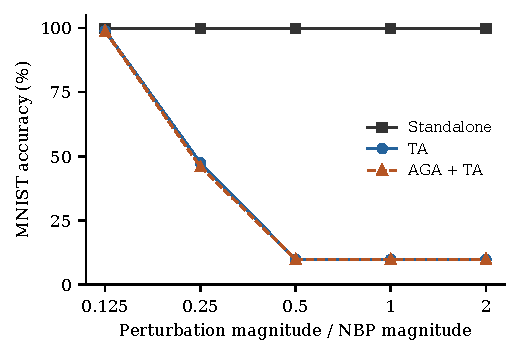
\includegraphics[width=\linewidth]{fig/amplitude.pdf}
\caption{Magnitude controls on the frozen MNIST perturbation, with SVHN as the companion. The horizontal axis rescales the published NBP update. Standalone accuracy is 99.69\% at all five magnitudes. Smaller updates at 0.125 and 0.25 retain substantial merged accuracy, while 0.5, 1, and 2 give 9.80\%. The released update corresponds to magnitude 1.}
\label{fig:amplitude}
\end{figure}
\Cref{fig:amplitude} varies only the update magnitude. At 0.125 of the NBP magnitude, MNIST accuracy after AGA and TA is 98.71\%; at 0.25 it is 45.88\%. The standalone predictions remain unchanged throughout the evaluated range.

\subsection{Multiple experts}
\Cref{tab:main} also reports eight-expert merging with TA coefficient 0.2, protecting one of the seven evaluated tasks at a time. All eight source experts participate in the author-specified order, including EuroSAT. After AGA, \method{} retains protected-task accuracies of 9.80\%, 6.70\%, and 2.13\% on MNIST, SVHN, and DTD, respectively; the corresponding scores are 2.44\%, 0.55\%, 1.19\%, and 0.25\% on RESISC45, Cars, GTSRB, and SUN397. AGA restores PaRaMS close to the matching unprotected result.

For each protected direction, we evaluate NBP and its unprotected control on all seven validated test sets. Thus the reported target-task entries are accompanied by a complete cross-task evaluation for these two methods. The coefficient $0.2$ multiplies each task update and gives the public base a coefficient of $1-8(0.2)=-0.6$ when written as a weighted sum of checkpoints.

\subsection{Fixed-readout analysis}
\begin{figure}[!t]
\centering
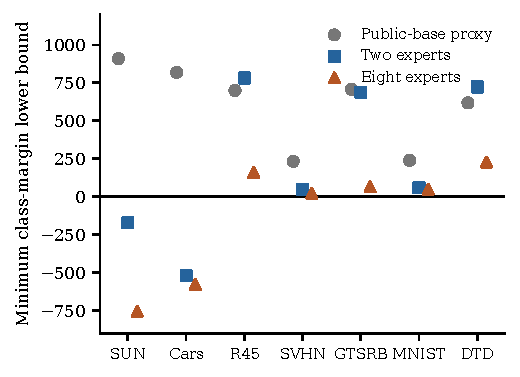
\includegraphics[width=\linewidth]{fig/readout_bound.pdf}
\caption{Minimum class-margin lower bound from \cref{eq:actualbound}, computed from the frozen NBP readout tensors. Positive values certify a constant prediction for every normalized hidden state in real arithmetic. Nonpositive values are inconclusive. SUN and R45 denote SUN397 and RESISC45. The public-base interpolation uses coefficient 0.5; actual two- and eight-expert TA use 0.5 and 0.2, respectively.}
\label{fig:readout}
\end{figure}
\Cref{fig:readout} examines seven frozen releases and their matching unprotected readouts in three settings, for 42 readouts in total. All seven protected public-base interpolations satisfy the bound. Five of seven actual two-expert models and five of seven actual eight-expert models also satisfy it. No matching unprotected model satisfies this sufficient condition. SUN397 and Cars do not satisfy it for the actual merges, despite their low measured accuracy; the sufficient bound does not describe every failure.

For the five certified tasks, modifying only earlier blocks cannot restore classification while keeping the stated readout fixed. This explains the measured failure of block-only alignment, final-MLP replacement, and the fixed ProDistill adaptation where applicable. It does not explain resistance to final-bias cleanup, which changes a parameter in the condition.

\subsection{A second vision backbone}
\begin{table}[!t]
\centering
\small
\setlength{\tabcolsep}{4pt}
\caption{CLIP ViT-B/16 protected-task accuracy (\%). The same NBP construction is applied to three experts. Two-expert TA uses coefficient 0.5; AGA processes the protected expert before merging.}
\label{tab:backbone}
\begin{tabular}{llrrr}
\toprule
Setting & Defense & MNIST & SVHN & DTD \\
\midrule
\multirow{2}{*}{Standalone} & None & 99.76 & 97.86 & 82.07 \\
 & \textbf{NBP} & 99.76 & 97.86 & 82.07 \\
\midrule
\multirow{2}{*}{TA} & None & 99.40 & 95.44 & 73.56 \\
 & \textbf{NBP} & 28.71 & 6.70 & 2.13 \\
\midrule
\multirow{2}{*}{AGA + TA} & None & 99.35 & 95.03 & 72.39 \\
 & \textbf{NBP} & 28.70 & 6.70 & 2.13 \\
\bottomrule
\end{tabular}
\end{table}

\Cref{tab:backbone} applies the same weight-only construction to CLIP ViT-B/16, whose final projection also has shape $768\times512$. All standalone predictions are preserved on the three full test sets. After AGA and TA, protected-task accuracy is 28.70\% on MNIST and 6.70\%/2.13\% on SVHN/DTD. Thus the effect transfers to this backbone, but MNIST does not reach the B/32 result. The AGA attention and MLP operations are unchanged and are applied to the B/16 architecture.

\subsection{Recovery at the final readout}
\label{sec:limitations}
\begin{table}[!t]
\centering
\small
\setlength{\tabcolsep}{4pt}
\caption{TA accuracy after public final-bias projection (\%). Columns give target (T) and companion (C) accuracy. Both releases receive the same cleanup before TA at 0.5. Their full prediction vectors are identical in these experiments.}
\label{tab:cleanup}
\begin{tabular}{lrrrr}
\toprule
Target & None T & None C & NBP T & NBP C \\
\midrule
MNIST & 99.37 & 92.50 & 99.37 & 92.50 \\
SVHN & 92.50 & 99.37 & 92.50 & 99.37 \\
DTD & 69.26 & 99.45 & 69.26 & 99.45 \\
\bottomrule
\end{tabular}
\end{table}

The preceding recovery procedures leave the final LayerNorm bias fixed. A method-specific attacker can instead remove its nullspace component using the published projection. For full-column-rank $P_e$, let $\Pi_e=P_e(P_e^{\mathsf T}P_e)^{-1}P_e^{\mathsf T}$. Then
\begin{equation}
 \begin{aligned}
 \Pi_e(b_e+\tau u)&=\Pi_e b_e,\\
 (\Pi_e b_e)^{\mathsf T}P_e&=b_e^{\mathsf T}P_e.
 \end{aligned}
 \label{eq:cleanup}
\end{equation}
This removes the added perturbation and preserves the standalone embedding, without data or the original expert. It need not recover the original bias itself. In the three-task experiment (\cref{tab:cleanup}), applying this operation to both NBP and its unprotected control gives identical merged predictions. No choice of magnitude or direction within the same kernel prevents this operation.

NBP therefore disrupts the evaluated merging and block-recovery procedures, but does not provide protection against arbitrary readout modification. Output calibration and student training in our additional recovery checks also restore accuracy. These outcomes distinguish the measured effect from a general white-box security claim.

\section{Conclusion}
A bias update in the expert projection's left nullspace preserves its standalone embedding and can be exposed by merging. NBP constructs this update from weights alone. The evaluated block-level procedures retain its effect, while final-bias projection removes it.
\clearpage
% The required LLM Usage Statement will be finalized with the authors before submission.
{\small
\bibliographystyle{ieeenat_fullname}
\bibliography{main}
}
\end{document}
